\chapter{Introduction} \label{chapter:1}

\section{Motivation} \label{section:GBM}
In financial econometrics, the geometric Brownian Motion (GBM) is the most popular method for describing the evolution of asset prices \citep*{hull1987pricing}. A random process $S_t$ follows geometric Brownian motion if it is the solution to the stochastic differential equation:
\begin{equation}
	dS_t = \mu S_t dt + S_t \sigma dW_t,
\end{equation}
where $W_t$ is a standard Wiener process and $\mu$ and $\sigma$ are the instantaneous drift and volatility of the process, respectively. Under the GBM, the increments of the log price $(Y_t \equiv \log S_t)$ over a period $\Delta$, which constitute the log returns of the asset, are independent, stationary, and identically distributed 
	\[ r_{t+\Delta} \equiv Y_{t + \Delta} - Y_t = \log(S_{t+\Delta}/S_t) \sim N\left( \Delta \mu, \Delta \sigma^2\right). \]

The use of GBM to model the evolution of asset prices facilitates estimation and pricing of financial derivatives. However, early work by \cite{mandelbrot1967variation} and \cite{fama1965behavior} showed that volatility changes over time. For example, Figure (\ref{fig:squared-log-returns}) shows the daily squared log returns $(r_{t + \Delta})^2$ for the S\&P 500 index and Netflix, Inc., along with simulated daily squared log returns generated with constant volatility. The non-constant volatility of the assets over time is evident by volatility clustering for the asset prices: the distinct periods of low and high daily squared log returns which, under constant intraday volatility and zero drift, have expected values equal the daily volatility. Empirical evidence also shows that negative returns tend to lead to higher volatility than positive returns, which is a phenomenon known as leverage. This chapter reviews models used to capture some of these stylized features of the data.

%
%\begin{figure}[h!]
%	\centering
%	\includegraphics[scale=0.8]{SP500-daily-squared-log-returns.pdf}
%	\caption{Daily squared log returns for the S\&P 500 index and Netflix, Inc. Evident in this figure is the clustering of periods with low and high daily changes in price, demonstrating that asset volatility fluctuates over time.}
%	\label{fig:SP500-daily-squared-log-returns}
%\end{figure}
%
\begin{figure}[htbp]
        \centering
        \begin{subfigure}[t]{0.4\textwidth}
                \includegraphics[width=\textwidth]{./chapter-1-introduction/SP500-daily-squared-log-returns.pdf}
                \caption{Daily squared log returns for the S\&P 500 index.}
                \label{fig:sp500-returns}
        \end{subfigure}%
        \quad %add desired spacing between images, e. g. ~, \quad, \qquad, \hfill etc.
          %(or a blank line to force the subfigure onto a new line)
        \begin{subfigure}[t]{0.4\textwidth}
                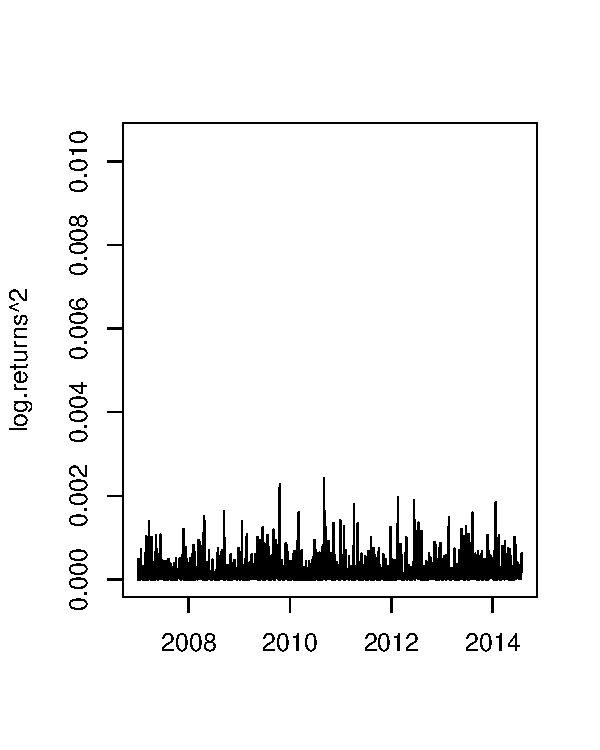
\includegraphics[width=\textwidth]{./chapter-1-introduction/SP500-daily-squared-log-returns-constant-vol.pdf}
                \caption{Simulated daily squared log returns, obtained by sampling a normal distribution with the mean and standard deviation of the S\&P 500 daily log returns. }
                \label{fig:sp500-returns-constant-vol}
        \end{subfigure}
	\\
	\begin{subfigure}[t]{0.4\textwidth}
                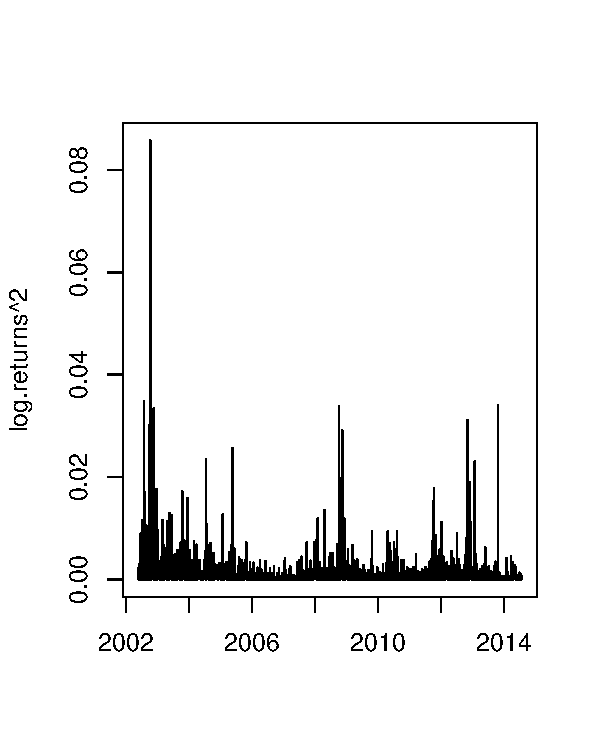
\includegraphics[width=\textwidth]{./chapter-1-introduction/Netflix-daily-squared-log-returns.pdf}
                \caption{Daily squared log returns for Netflix, Inc.}
                \label{fig:netflix-returns}
        \end{subfigure}%
        \quad %add desired spacing between images, e. g. ~, \quad, \qquad, \hfill etc.
          %(or a blank line to force the subfigure onto a new line)
        \begin{subfigure}[t]{0.4\textwidth}
                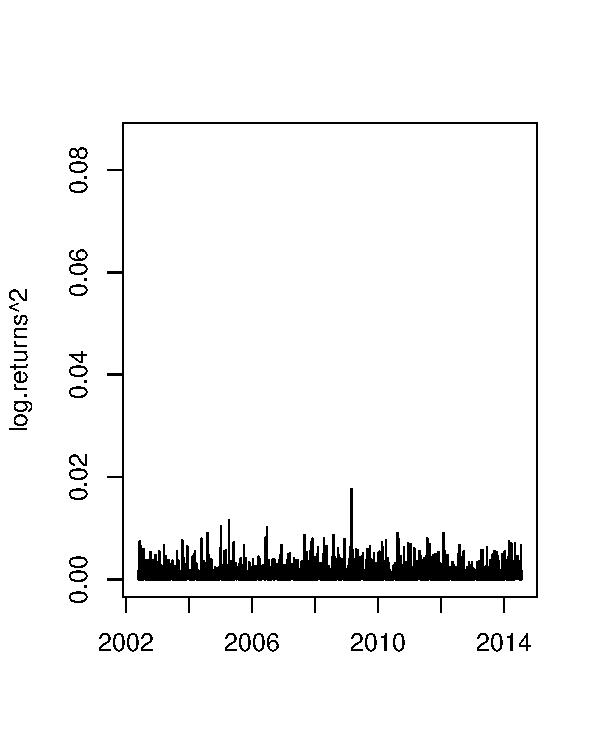
\includegraphics[width=\textwidth]{./chapter-1-introduction/Netflix-daily-squared-log-returns-constant-vol.pdf}
                \caption{Simulated daily squared log returns, obtained by sampling a normal distribution with the mean and standard deviation of the Netflix, Inc. daily log returns. }
                \label{fig:netflix-returns-constant-vol}
        \end{subfigure}
	\caption{Evident in the above figures is the clustering of periods with low and high daily changes in price for the market data, demonstrating that asset volatility fluctuates over time. The constant volatility simulated data is characteristically different from the market data.}
	\label{fig:squared-log-returns}
\end{figure}

\section{Review of Models for Time-varying Volatility}
The literature on volatility as a non-constant process ranges from the early autoregressive 
heteroskedastic (ARCH) model by \cite{engle1982} and the generalized version by \cite{bollerslev1986},
to stochastic volatility models \citep*{hull1987pricing}. Most statistical models 
have used opening and closing prices over the frequency considered for estimation and forecasting.

	\subsection{ARCH/GARCH Models}
	The most important development in modeling volatility changes has been the \textit{autoregressive conditional heteroskedasticity} or ARCH model, introduced by \cite{engle1982}. In results from models of inflation, Engle found that large and small forecast errors occurred in clusters, suggesting a form of heteroskedasticity in which the variance depends on the size of previous fluctuations. 

We will introduce ARCH models with the particular ARCH($p$) model. ARCH models use a conditional structure to model time-varying volatility. Assuming that the log returns $r_t$ follow the linear relationship
\begin{align*}
r_t &= \mu + \epsilon_t, &  t=1,\ldots, T, \\
\epsilon_t &\sim N(0, \sigma_t^2)
\end{align*}
%
where $\mu$ is a mean level that may be dependent on regression and explanatory variables, the ARCH($p$) model characterizes the distribution of the stochastic error by imposing an autocorrelated, time-dependent structure on the variance of the noise term
\begin{eqnarray*}
	\sigma_t^2 &=& \omega + \sum_{i=1}^p \alpha_i \epsilon^2_{t-i}, \\
	\epsilon_t &=& \sigma_t Z_t,
\end{eqnarray*}
where $\omega$ and $\{ \alpha_i \}, i=1,\ldots, p$ are nonnegative constants, and $Z_t \sim N(0,1)$. The conditional variance function is formulated to mimic the phenomenon of large volatility following large shocks to the dependent variable manifested as large deviation of $r_t$ from the mean $\mu$. In other words, high value for $\epsilon_t^2$ increases $\sigma^2_{t+1}$, which in turn increases the expectation of $\epsilon_{t+1}^2$, and so on. 

\cite{bollerslev1986} extended the ARCH($p$) model into the GARCH($p,q$) model, the \textit{generalized} ARCH, by including past variances into the conditional variance formula:

	\[ \sigma_t^2 = \omega + \sum_{i=1}^q \alpha_i \sigma^2_{t-i} + \sum_{i=1}^p \beta_i \epsilon^2_{t-i}. \]
%
This additional feature captures longer-term effects outlasting the impacts of shocks to the dependent variables. One issue is that, if $\alpha_i$ and $\beta_i$ are left unrestricted, the variance can potentially be negative. 

ARCH and GARCH models have been widely successful \citep*{bollerslev2003measuring}, but they fail to capture some important features of financial and economic data. The most important feature not captured is the leverage effect, which has been addressed by Nelson's \textit{exponential} GARCH \citep*{nelson1991conditional} model: 

 	\[ \log \sigma_t^2 = \omega + \sum_{i=1}^p \alpha_i \log \sigma_{t-i}^2 + \sum_{i=1}^q \beta_i g(Z_{t-i}), \]
where 
	\[ g(Z_t) = \theta Z_t + \gamma[ |Z_t| - E|Z_t| ], \] 
with $Z_t \sim N(0,1)$. Assuming that $\gamma > 0$ and $\theta = 0$, the innovations in $\log \sigma^2_{t+1}$ are positive (negative) when the magnitude of $Z_t$ is larger (smaller) than its expected value. If $\gamma = 0$ and $\theta <0$, the innovation in the variance is negative (positive) when $Z_t$ is positive (negative). In this manner the EGARCH model captures the asymmetric leverage effect of negative returns leading to greater volatility, as well as the previously included effect of above (below)-average (in terms of magnitude) residuals leading to greater (smaller) volatility. 

ARCH-type models are appealing because they allow for direct parametric modeling of volatility, and consequentially varieties of models building upon the ARCH, GARCH, and EGARCH models presented so far have been developed. The immediate availability of a conditional likelihood function for the observables allows for standard and efficient MLE methods to be used for fitting \citep*{baillie1991bivariate}, and by an extension, Bayesian analysis is applicable as well \citep{bauwens1998bayesian, nakatsuma2000bayesian, vrontos2000full}. 


	\subsection{Stochastic Volatility}
	Whereas GARCH uses a single stochastic process to drive both the asset and volatility process, stochastic volatility (SV) models are defined by a set of two stochastic differential equations that define separate (but possibly dependent) evolutions for the asset and volatility:
\begin{eqnarray}
	dS_t &=& \mu(S_t, \sigma_t)dt + \nu(S_t, \sigma_t)dW_{t,1} \label{eq:SV-model-1}, \\
	d\sigma_t &=& \alpha(S_t, \sigma_t)dt + \beta(S_t, \sigma_t)dW_{t,2}, \label{eq:SV-model-2}.
\end{eqnarray}

One of the first and most well-known continuous-time SV models was introduced by \cite{hull1987pricing}. In it, the log price follows Brownian motion (so that the price follows GBM) with changing volatility, and the volatility follows an Ornstein-Uhlenbeck (OU) process:
	\begin{eqnarray*}
			d Y_t &=& \mu dt + \sigma_t dW_{t,1} \\
			d \log( \sigma_t ) &=& \alpha(\phi - \log(\sigma_t))dt + \omega dW_{t,2} 
	\end{eqnarray*}

Discretizing the continuous-time model above produces the state-space model
\begin{align*}
	Y_t 			&= \mu + Y_{t-1} + \epsilon_t^1 								 & \epsilon_t^1 \sim N(0, \sigma_t^2), \\
	\log(\sigma_t) &= \alpha + \phi \left[ \log(\sigma_{t-1}) - \alpha \right] + \epsilon_t^2  & \epsilon_t^2 \sim N(0, \tau^2),
\end{align*}
which is the model proposed by \cite{clark1973subordinated}, one of the first papers in which serial correlation is allowed in the volatility process.  

%Expressed in integral form, the standard SV model becomes 
%	\begin{eqnarray}
%		S_t =  S_0 + \int_0^t \mu(S_s, \sigma_s) ds + \int_0^t \nu(S_s, \sigma_s) dB_{s,1} \\
%		\sigma_t = \sigma_0 +  \int_0^t \alpha(S_s, \sigma_s) ds + \int_0^t \beta(S_s, \sigma_s) dB_{s,2}
%	\end{eqnarray}

%	One of the first papers on SV that does allow for serial correlation is by Taylor (1982) who introduced his model in the discrete time setting. The risky part of returns was modeled as the process
%	\[ m_i = M_i - M_{i-1} = \int_{t_i}^{t_{i+1}} \sigma_s dW_s = \sigma_i \epsilon_i. \]
%It was assumed that $\sigma_i$ and $\epsilon_i$ are independent, and that $\epsilon$ has mean zero and unit variance. Hence, $\sigma_i$ can be thought of as the variance of the random process, allowed to vary from timestep to timestep. The change of $\sigma_i$ over timesteps is modeled with autoregressive process
%	\begin{eqnarray*}
%		\sigma_i &=& \exp(h_i/2) \\
%		h_{i+1} &=& \mu + \phi(h_i - \mu) + \nu_i
%	\end{eqnarray*}
%	where $\nu_i$ is Gaussian with zero mean and unit variance. If $\epsilon_i$ is assumed to be Gaussian, this is the log-normal model. The general formulation above allows for direction of returns to influence future volatility by correlating $\epsilon$ and $\nu$. This captures the important empirically observed leverage effect.

%One mathematically tractable and widely used parameterization of the general form of SV models is where the price follows GBM with changing volatility, and the volatility follows an Ornstein-Uhlenbeck (OU) process
%\begin{eqnarray*}
%	dY_t &=& \mu dt + \sigma_t dB_{t,1} \\
%	d\log(\sigma_t) &=& \kappa(\theta - \log(\sigma_t)) + \tau dB_{t,2}.
%\end{eqnarray*}

%One of the first and most well-known continuous-time SV model was introduced by Hull and White \cite{hull1987pricing} in 1987. They proposed two continuous time SV model, the latter one being:
%	\begin{eqnarray*}
%			d \log(Y_t) &=& \mu(Y_t, t) dt + \sigma(Y_t, t) dW_t \\
%			d \log( \sigma^2 ) &=& \alpha(\mu - \log(\sigma^2))dt + \omega dB 
%	\end{eqnarray*}
%where $\omega(\cdot)$ is a non-negative deterministic function and $B$ is a second Brownian motion. Discretization of this model produces the model suggested by Taylor. 

From the late 1990s, stochastic volatility models have taken center stage in econometric analysis of volatility forecasting \citep*{shephard2005selected-readings}. Stochastic volatility models can capture time clustering \citep*{hull1987pricing}, as well as leverage effects \citep*{yu2005leverage} by introducing correlation between $W_{t,1}$ and $W_{t,2}$. 

Empirical evidence suggests that, across different asset types and timescales, the dependence in the volatility structure initially decays quickly at short lags but then decays slowly at longer lags \citep*{andersen1997heterogeneous, andersen1997intraday, andersen1998answering}. For this reason, effort has been placed on developing both continuous and discrete-time long-memory SV models. In the discrete case, one approach has been to model log volatility as a fractionally integrated process \citep*{harvey2002long, breidt1998detection-estimation}. In continuous time, the log volatility has been modeled as fractionally integrated Brownian motion \citep*{comte1998long}, and a square root model driven by fractionally integrated BM \citep*{comte2012affine}. Another important extension includes the addition of jumps in the diffusion of price \citep*{bates1996jumps}. 

Fitting stochastic volatility models is made difficult by the non-linearities of the likelihood as well the large sample space formed by the latent series $\{ \sigma_t \}$. Techniques for estimation of SV models include quasi-maximal likelihood approaches as done by \cite{ruiz1994quasi}, the particle filter approach of \cite{sandmann1998estimation}, the generalized method of moments \citep*{melino1990pricing}, and MCMC methods \citep*{jacquier2002bayesian, kim1998stochastic, omori2007stochastic}.

	\subsection{ Time-changed Brownian Motion}
	A more general approach for representing changing volatility in financial assets, which encompasses both stochastic volatility and GARCH-type models, is time-changed Brownian motion. Time-changed Brownian motion was first used in the paper of \cite{clark1973subordinated}, which introduced the concept into financial economics. Under time-changed Brownian motion, the log-price $Y$ of an asset is written as 
	\begin{equation}
		Y_t = W_{\tau_t}, \quad t \geq 0,
	\end{equation}
	where $W$ is Brownian motion, $t$ is continuous time and $\tau_t$ is a non-negative process with non-decreasing sample paths. If $W$ and $\tau$ are independent, $Y_t | \tau_t \sim N(0, \tau_t)$. In this case, it is immediately obvious that this formulation allows for the second moments of the price process to change over time. Further, marginally $Y_t$ is a scale mixture of normals, which means that returns are symmetric but can be fat tailed. The time-change process $\tau_t$ can be modeled as either a function of some observables, or as a latent process, which is more in line with the modern development of stochastic volatility. 

Time-changed Brownian motion has also become a popular tool for building financial models \citep*{geman2005measure}. Stochastic processes of this kind can capture asset price jumps, changing return volatility, and correlation between volatility and asset returns \citep*{carr2004time}. The mathematical treatment of these models usually involves the computation of the characteristic function, which is typically easy to get as long as $\tau$ and $W$ are independent. However, even if the characteristic function is available in closed form, the associated density often needs to be computed numerically.

%Since the work of Heston \cite{heston1993closed}, focus has been placed on the use of characteristic functions for understanding proposed processes. A closed-form expression for the characteristic function allows for a closed-form expression for the probability density of the underlying asset price. Such a likelihood function can be used to find MLE for model parameters, as well as for evaluating option prices.
%However, Clark's paper did not allow for serial correlation of increments of $\tau_t$ that would generate clustering in $M$. 
%	Putting Clark's paper in a more modern context, as long as $E(\sqrt{\tau_t}) < \infty$, he modeled the ``risky'' part of a semimartingale 
%	\[ Y = A + M, \]
%where the increments of $A$ is the reward component compensating the investor for taking on the risky component $M$. Conditioning on the time-change process $\tau_t$, we have 
%	\[ Y_t | \tau_t \sim N( f(\mu, t, \tau_t), \tau_t), \]
%where $\mu$ is some vector of parameters. We see that this is the more general version of the solution to the stochastic differential equation (\ref{eq:SDE-geo-BM}). 

%	\section{Range-Based Estimation}
%	As we saw in the previous section, realized variance is a ex-poste volatility estimator that can be used to fit continuous (through GMM) and discrete-time (state-space representation) SV models. To improve model fitting and estimation for SV models, we can use the price range within a sampling interval $\Delta$ for an asset, as in \cite{alizadeh2002range}. We denote the range-based statistic as $f(S_{i\Delta}, S_{(i+1)\Delta})$, again where $S_t$ is the price of the asset. If the estimator is homogeneous in the volatility, we write
%\[ f(S_{i\Delta}, S_{(i+1)\Delta}) = \sigma_{i\Delta}^\gamma f(S^*_{i\Delta}, S^*_{(i+1)\Delta}), \]
%where $S^*_t$ is the standarized diffusion. 
%Hence, if the latent volatility follows an OU-process, we can write the state-space model 
%\begin{eqnarray*}
%	\log(\sigma_{(i+1)\Delta}) &=& \alpha + \phi \left[ \log(\sigma_{(i-1)\Delta}) - \alpha \right] + \epsilon_{(i+1)\Delta}\\
%	\log\left| f(S_{i\Delta}, S_{(i+1)\Delta}) \right| &=& \gamma \sigma_{(i+1)\Delta} + E\left( \log\left| f(S^*_{i\Delta}, S^*_{(i+1)\Delta}) \right| \right) + \nu_{(i+1)\Delta},
%\end{eqnarray*}
%where $\sigma_{i\Delta}$ is the assumed constant volatility over $\Delta$. This can be estimated, once more, with a Kalman filter. The usefulness of this approach lies in that we can use different estimators for the volatility $f(S_{i\Delta}, S_{(i+1)\Delta})$, and that the dynamical model form is convenient and efficient to use for both estimation and prediction. 

\section{Time-Varying Volatility in High-Frequency Data}
The advent of electronic trading has allowed for the increase in the volume and speed at which transactions on financial markets are performed and recorded. Today, transactions occur on a microsecond timescale \citep*{brogaard2010high} for certain types of assets, and there has been increasing interest in using this data to better understand volatility in financial markets. 

Much of the effort to use high-frequency data to understand the evolution of volatility has focused on \textit{realized volatility}. The concept of realized volatility was introduced in three independent papers by \cite{andersen2001distribution}, \cite{barndorff2002estimating}, and \cite{comte1998long} as a means to perform the estimation of $\int_t^{t+\Delta} \sigma^2(Y_s, s) ds$, where $\Delta$ is some finite period of time and $y_t$ is the log-price of the asset following a diffusion process. 

Let $\Delta = 1$ day, and suppose there are $m$ observation of the price over the trading period. The $i^{th}$ interday log-return is defined as 
\begin{align*}
r_i^{(m)} &= y_{i/m} - y_{(i-1)/m}, &  i =1, \ldots, m.
\end{align*}

The sum of the squared log intraday returns is the realized volatility
\begin{equation}
	RV^{(m)} = \sum_{i=1}^m r_i^{(m)^2}. \label{eq:RV}
\end{equation}
It can be shown that $RV^{(m)} \xrightarrow{p} \int_t^{t+\Delta} \sigma^2(Y_s, s)ds$ as $m \to \infty$. Realized volatility is a consistent estimator of the integrated volatility \citep*{barndorff2002econometric}, and it is asymptotically distributed:
\begin{equation}
 \frac{\sqrt{m} (RV^{(m)} - \int_{t}^{t+\Delta} \sigma^2(Y_s,s)ds)}{\sqrt{ 2\int_{t}^{t+\Delta} \sigma^4(Y_s,s)ds} } \xrightarrow{d} N(0,1) \label{eq:asy}
\end{equation}

\cite{barndorff2004power} also propose a consistent estimator for the power variation $\int_{t}^{t+\Delta} \sigma^4(y_s,s)ds$, which is needed to construct credible confidence intervals given the result in equation (\ref{eq:asy}). There has been further work in the derivation of consistent estimators of higher moments of the integrated volatility, which are used in the estimation of continuous time SV models with higher frequency data \citep*{todorov2011econometric}.

%The realized volatility estimator is a nonparametric estimator with very desirable asymptotic properties, given that the assumptions on the diffusion process for the log-price hold. Yet one problem with using RV alone is that it can only estimate the integrated volatility over $\Delta$. In other words, practitioners can use RV as a stand-alone tool to at best estimate the average of the volatility process over the sampling period. 

	\subsection{Microstructure Noise}
One challenge with the analysis of high-frequency price data is the presence of microstructure noise at the microsecond timescale. As the sampling period shrinks down to the transaction-by-transaction frequency, irregular spacing between transactions, discreteness in transaction prices, and very short-term temporal dependence become dominant features of the data \citep*{stoll2000presidential}. For this reason, the foundational diffusion assumption on the log-price of assets no longer holds. Measurements at high frequencies no longer capture only the evolution of prices, but they capture a noisy version of the price. 

In the model-free setting of realized volatility estimators, one approach to mitigating the confounding effects of microstructure noise is to combine averaged RV estimates obtained by subsampling the data with a RV estimate using all available data \citep{zhang2005tale}. Another approach is to employ a class of kernel-based methods similar to those used for estimating the long-run variance of a stationary time-series in the presence of autocorrelation \citep{hansen2006realized}. 

In the context of stochastic volatility, microstructure noise could, for example, be accounted for with a model of the form:
\begin{eqnarray*}
	Y_{t+1} &=& \log(S_{t+1}) + m_{t} \\
	\log(S_{t+1}) &=& \log(S_{t}) + \mu(S_t, \sigma_t) + \nu(S_t, \sigma_t)\epsilon_{t+1,1} \\
	\log(\sigma_{t+1}) &=& \log(\sigma_{t}) + \alpha(S_t, \sigma_t) + \beta(S_t, \sigma_t)\epsilon_{t+1,2}.
\end{eqnarray*} 
The distributional assumptions on the noise $m_t$ can be varied, and there can be correlation between the innovation terms $\epsilon_{t+1,1}$ and $\epsilon_{t+1,2}$
%
%For the above-mentioned reasons, the realized volatility estimator is often used as part of an inferential model.

	\subsection{Stochastic Volatility Models and High-frequency Data} \label{sec:stoch-vol-models-and-high-freq-data}
One of the first papers to use realized volatility in the estimation of continuous-time SV models is by \cite{barndorff2002econometric}. The idea of the paper is use the continuous time SV model and the RV estimator to form a state-space model, which can be estimated with a Kalman filter.

Assuming the variance $\sigma^2(t)$ follows the Ornstein-Uhlenbeck (OU) process instead of the log-variance, the autocorrelation function for the volatility is known to be $r(t, t') = \exp(-\lambda \left| t' - t \right|)$. The functional form for $r(t)$ allows for the explicit form of the correlation function between observations in the volatility process:
%
\[ corr(\sigma^2_{t}, \sigma^2_{t+s}) = d \exp(t\{ -\lambda\Delta(s-1) \}), \]
%
where $d$ is a constant in terms of $\lambda$ which is less than 1, and $\Delta$ is the length of time between returns. Hence, the actual volatility has the autocorrelation function of an autoregressive moving average (ARMA) model of order (1,1). Letting $RV^{(m)}_t$ be the realized volatility in interval $(t-\Delta, t)$ computed with $m$ intraperiod observations, $RV^{(m)}_t$ can be decomposed in terms of the true volatility for the interval plus an error term $u_t$ due to microstructure noise
\begin{equation}
	RV^{(m)}_t = \sigma^2_t + u_t. \label{eq:decomposition}
\end{equation}
Setting $E(\sigma^2_t) = \xi \Delta$, and using the ARMA(1,1) representation of the volatility process, equation (\ref{eq:decomposition}) becomes
\[
	RV^{(m)}_t = (\xi \Delta + \phi \sigma^2_{t-1} + \theta \sigma_{\sigma}\epsilon_{t-1} + \sigma_{\sigma}\epsilon_{t} ) + (\sigma_u \nu_t),
 \]
where $\epsilon_{t-1}, \epsilon_t, \nu_t \sim N(0,1)$. The parameter $\sigma_{\sigma}$ is the standard deviation of the innovations driving the volatility process, $\sigma_u$ is the standard deviation of the microstructure noise, and $(\phi,\theta)$ are the ARMA parameters. Therefore, the realized volatility observations can be expressed as the state-space model
\begin{eqnarray*}
	RV^{(M)}_t &=& \Delta \xi + (1 \quad 0 )\alpha_t + \sigma_u v_{t} \\
	\alpha_{t} &=& \left( \begin{array}{cc} \phi & 1 \\ 0 & 0 \end{array} \right) \alpha_{t-1} + \left( \begin{array}{c} \sigma_\sigma \\ \sigma_\sigma \theta \end{array} \right) \epsilon_{t},
\end{eqnarray*}
which can be estimated with a Kalman filter.

An alternative approach for estimating SV models using realized volatility data is based on the generalized method of moments. In this method, higher powers of realized volatility are used as approximations to higher orders of integrated volatility, as done by \cite{bollerslev2002estimating}. By matching the sample moments of the realized volatility to the moments of the integrated volatility implied by the continuous-time SV model, a generalized method of moments estimator for the underlying model parameters can be obtained. Some more recent works dealing with fitting stochastic volatility models to high-frequency data include that of \cite{venter2012extended} and \cite{shirota2014realized}.

\section{Plan for the Advancement}
In Chapter \ref{chapter:2} we will derive the likelihood for closing prices of financial asset prices that takes into account the highest and lowest prices within a trading period. We also compare maximum likelihood estimates for volatility based on this approach to realized volatility estimates using simulated high-frequency data. In Chapter \ref{chapter:3} we extend the model in Chapter \ref{chapter:2} to two dimensions and examine the convergence properties of the thus-derived likelihood solution. In Chapter \ref{chapter:4} we outline the future direction of this project. 

%In the general setting of (\ref{eq:SV-model-1}) - (\ref{eq:SV-model-2}), the estimation of volatility parameters based on the discretely sampled observations is complicated by the $\sigma(t)$ process being latent. However, as already discussed, realized volatility approximates almost surely $\int_t^T \sigma^2(s)ds$ as the sampling frequency increases. Hence, explicitly treating the integrated volatility as observable allows the implementation of generalized method of moments-like estimators. 

%Considering the model 
%\begin{eqnarray}
%	dY_t &=& \sqrt{V_t}dB_t \\
%	dV_t &=& \kappa(\theta - V_t)dt + \sigma\sqrt{V_t}dW_t, 
%\end{eqnarray}
%the authors develop the conditional expectations for the integrated volatility $\int_{t+1}^{t+2} V_s ds$ and integrated variance $\int_{t+1}^{t+2} V^2_s ds$, given a filtration $G_t$ up to time $t$:
%\begin{eqnarray*}
%	E\left( \int_{t+1}^{t+2} V_s ds | G_t \right) &=& \alpha E\left( \int_{t}^{t+1} V_s ds | G_t \right) + \beta, \\
%	E\left( \int_{t+1}^{t+2} V^2_s ds | G_t \right) &=& H E\left( \int_{t}^{t+1} V^2_s ds | G_t \right) + I E\left( \int_{t}^{t+1} V_s ds | G_t \right) + J,
%\end{eqnarray*}
%with $H, I$, and $J$ being defined in terms of the model parameters. The analytical solutions for the conditional first and second moments allow for the construction of a standard GMM estimator for the model parameters. 

%	\subsection*{Non-equally spaced observations}
%	Financial transaction data inherently arrive in irregular time intervals in the form of bid and ask offers of market traders. Frequently traded stocks will have transactions every few seconds, while commodities will have transactions every day or even every week. If a short interval is chosen for econometric analysis, there will be many intervals with no new information and heteroskedasticity will be introduced into the data, yet if a lzonger interval is chosen multiple  transactions will be averaged and potential covariate relationships in the data will be lost, thereby making high-frequency data not extra advantageous. What complicates the choice of a best time intervals for econometric analysis is that the rate of transaction arrival within any chosen fixed interval may vary over its course, and also that any asset traded may randomly exhibit unusual activity due to an unobservable event (with respect to the asset price). 

%	An alternative to fixed interval analysis is proposed in \cite{engle1998autoregressive} with the autoregressive conditional duration model (ACD). The arrival times of market events, such as price changes and volume of trade offers, are represented as random variables following a self-exciting point process, where the means of arrival time intervals are modeled as an ARMA process. Each arrival interval is then represented by its expected duration times an innovation term, which in this paper is the Weibull distribution. The intensity of arrivals is a baseline function multiplied by a normalized current time interval with respect to the conditional expected duration. The baseline intensity is modeled semi-parametrically and inter-day trading effects are included. The model is used to estimate and forecast the intensity of transaction arrivals and hence get an estimate of instantaneous volatility, as well as test hypotheses about market microstructure. This model is used in \cite{russell1998}, where additionally conditional, discrete price transition probabilities are developed. 

%	Their approach has been subsequently extended by many authors. Bauwens and Giot [3] put forth a log-linear specification for the conditional mean which always guarantees the positivity of the durations without imposing restrictions on the coefficients. Zhang et al. [25] introduced a non-linear version of the ACD model in the spirit of the linear autoregressive threshold models. Bauwens and Veredas [5] proposed a stochastic duration model which is analogous to the stochastic volatility models in the same way as the Engle and Russel’s ACD model is analogous to the GARCH model. Ghysels et al. [14] considered a rather complicated version of the ACD model, which allows disentangling the dynamics of the mean and the variance of the duration process. In addition to the exponential and Weibull distributions for the error terms, other distributions have been proposed. Grammig and Maurer [16], and Grammig and Wellner [17] consider the Burr distribution and Lunde [20] considers the generalized gamma distribution. The log-normal distribution, although seemingly a natural candidate, has received limited attention in the literature with the exception of the work by Allen et al. [2] and Sun et al. [24]. Despite this impressive body of work, only a limited number of papers have been devoted to testing the specifications of the alternative ACD models. Two notable exceptions are the work of Fernandes and Grammig [13] and Bauwens et al. [4]. The first paper evaluates ACD models by gauging the distance between the parametric density of the duration process and its non-parametric estimate, using the methods developed by Ajt-Sahalia1 [1]. Only the standard ACD specification of Engle and Russel1 [11] is considered, using error terms with exponential,Weibull, generalized gamma and Burr distributions. Employing only one sample of durations for Exxon, these authors find that the Burr and generalized gamma distributions perform better than the exponential and Weibull distributions. Bauwens et al. [4], using the methodology for evaluating density forecasts by Diebold et al. [9], consider a number of alternative ACD specifications for three stocks traded on New York stock exchange. One of their main findings is that the exponential and Weibull distributions are often mis-specified, while on the other hand Burr and generalized gamma distributions perform much better. Additionally, they find that the specification for the conditional mean (e.g. the standard ACD, log-ACD as well as non-linear approaches such as the Threshold ACD model) does not seem to affect the models’ performance much. In particular, their results suggest very little difference between the ACD and log-ACD specifications.


%We also aim use the range of the asset price over $\Delta$, but by formally incorporating the information within the likelihood model that is given by assumption that log-price, $Y_t$, follows a diffusion process. Assuming that $\sigma$ is constant over the period of interest, the log-price follows the SDE
%\begin{equation}
%	dY_t = \mu dt + \sigma dW_t, \label{eq:SDE}.
%\end{equation}
%Using the Fokker-Planck Equation, we can take the SDE in (\ref{eq:SDE}) and express the probability density of the asset price $f(y,t)$ as the PDE
%\begin{eqnarray*}
%	\frac{\partial}{\partial t} f(y,t) &=& -\mu \frac{\partial}{\partial y}f(y,t) + \frac{1}{2}\sigma^2 \frac{\partial^2}{\partial y^2} f(y,t), \\
%	f(y,0) &=& \delta(y-y_0),
%\end{eqnarray*}
%where $y_0$ is the price at the beginning of the interval.
%The function $f(y,t)$ is the probability that $Y_t = y$, namely that the log-price of the asset is $y$ at time $t$. Without any additional restrictions, therefore, for any time period $\Delta$, we have the likelihood of a closing price, given the parameters $\mu$ and $\sigma$. Now, we incorporate the information that, for the observed path of the process, $\max\left\{ y \right\} = A$ and $\min\left\{ y \right\} = a$. Since $f(y,t)$ is the probability distribution of the price at time $t$, and $y(t)$ is the realization of the underlying stochastic process, in just the same way $A$ and $a$ are the realizations of the maximum and mininum of the process up to time $t$.  Hence, we can impose the condition that the maximum of the process $\sup\left\{ Y_t \right\}$ must, in general, be below $A$ and the minimum of the process $\inf\left\{ Y_t \right\}$ must exceed $a$. With the max/min information, the diffusion process SDE is modified to 
%\begin{equation}
%	dY_t = \mu dt + \sigma dW_t, \qquad \sup\left\{ Y_t \right\} \leq A \quad \inf\left\{ Y_t \right\} \geq a.
%\end{equation}
%In terms of the probability density, the SDE is now
%\begin{eqnarray}
%	\frac{\partial}{\partial t} f(y,t) &=& -\mu \frac{\partial}{\partial y}f(y,t) + \frac{1}{2}\sigma^2 \frac{\partial^2}{\partial y^2} f(y,t) \label{eq:IC-BV-1}\\
%	f(y,t) \leq A && f(y,t) \geq a, \qquad f(y,0) = \delta(y-y_0). \label{eq:IC-BV-2}
%\end{eqnarray}
%The solution to the IC/BV problem is interpreted as 
%\[ f(y,t) = P( \inf\{Y_t\} \geq a, \sup\{Y_t\} \leq A, Y_t = y | Y_0 = y_0 ). \]
%Thus, 
%\[ -\frac{\partial^2}{\partial A \partial a} f(y,t) = P( \inf\{Y_t\} = a, \sup\{Y_t\} = A, Y_t = y | Y_0 = y_0 ). \]
%The probability density function above is very important, as its maximization over the parameters $\mu$ and $\sigma$ produces maximum likelihood estimates $\hat{\mu}$ and $\hat{\sigma}$, which incorporate the max/min information over the period $\Delta$. MLE estimates are consistent and efficient, so that the estimators based on the solution to the IC/BV problem above will outperform other ad-hoc range-based estimators.

%\subsection*{Solution to the IC/BV Problem}
%The solution to the problem in (\ref{eq:IC-BV-1}) - (\ref{eq:IC-BV-2}) begins with a change of coordinates which transforms the advection-diffusion problem to a purely diffusion problem. Let 
%\[ f(y,t)=  \exp(ay + bt)u(y,t), \]
%so that 
%\begin{eqnarray*}
%	\frac{\partial}{\partial t} f(y,t) &=& -\mu \frac{\partial}{\partial y} (\exp(ay + bt) u(y,t)) + \frac{1}{2}\sigma^2\frac{\partial^2}{\partial y^2} (\exp(ay + bt) u(y,t)) \\
%		&= & -\mu \left[ a \exp(ay + bt) u(y,t) + \exp(ay + bt) \frac{\partial}{\partial y} u(y,t)  \right] \\
%		&& + \frac{1}{2}\sigma^2 \left[ a^2 \exp(ay + bt) u(y,t) + a \exp(ay + bt) \frac{\partial}{\partial y} u(y,t) + \exp(ay + bt) \frac{\partial^2}{\partial y^2} u(y,t) \right] \\
%		&=& u(y,t)\left[ -\mu a + \frac{1}{2}\sigma^2 a^2 \right] \exp(ay+bt) \\
%		&& + \frac{\partial}{\partial y} u(y,t)\left[ -\mu + \frac{1}{2}\sigma^2 a \right]\exp(ay+bt) \\
%		&& + \frac{\partial^2}{\partial y^2} u(y,t) \left[ \frac{1}{2}\sigma^2 \right] \exp(ay+bt) \\
%		&=& b\exp(ay+bt)u(y,t) + \exp(ay+bt)\frac{\partial}{\partial t}u(y,t) 
%\end{eqnarray*}

%We thus have the condition
%\begin{equation}
%	u(y,t)\left[ -\mu a + \frac{1}{2}\sigma^2 a^2 \right] + \frac{\partial}{\partial y} u(y,t)\left[ -\mu + \frac{1}{2}\sigma^2 a \right] + \frac{\partial^2}{\partial y^2} u(y,t) \left[ \frac{1}{2}\sigma^2 \right] = bu(y,t) + \frac{\partial}{\partial t}u(y,t) 
%\end{equation}
%The system 
%\begin{eqnarray*}
%	-\mu a + \frac{1}{2}\sigma^2 a^2 &=& 0 \\
%	b &=& 0
%\end{eqnarray*}
%defines $a = \sqrt{2\mu}/\sigma$, and $b=0$ such that the original problem is reduced to the heat equation on a bounded domain, with the same IC/BV conditions:
%\begin{eqnarray*} 
%\frac{\partial}{\partial t}u(y,t) &=& \frac{1}{2}\sigma^2 \frac{\partial^2}{\partial y^2} u(y,t) \\
%					u(y,t) &=& 0, \quad \mbox{for} \quad y = a, A \\
%					u(y,0) &=& \delta(y-y_0)
%\end{eqnarray*}

%We can solve the given problem with a Fourier-series representation of the solution:

%\begin{equation} 
%	u(y,t) = \sum_{n=1}^\infty a_n(t)\sin\left( \frac{n \pi (y+a)}{L_y} \right), \quad L_y = A-a \label{eq:trig-exp}
%\end{equation}

%We choose the collection of the odd trigonometric functions as a basis for the solution because they preserve the boundary conditions under the spatial differential operator, and they form a complete basis for solutions to the PDE. 
%Substituting (\ref{eq:trig-exp}) into the PDE produces a differential equation of the time-dependent coefficients:
%\[
%	\dot{a}_n(t)\sin\left( \frac{n \pi (y+a)}{L_y} \right) = - \left( \frac{n\pi}{L_y} \right)^2 a_n(t)\sin\left( \frac{n \pi (y+a)}{L_y} \right)
%\]
%Therefore, the expression for the coefficients is 
%\begin{equation}
%	a_n(t) = a_{n,0} \exp\left( - \left( \frac{n\pi}{L_y} \right)^2 t \right) ,
%\end{equation}
%where $a_{n,0}$ is the coefficient for the sine series representation of the initial condition $\delta(y-y_0)$. Having obtained the solution, we can take derivatives with respect to the max and min values $a, A$ in order to obtain an expression for the likelihood. 